\chapter*{Appendices}
\addcontentsline{toc}{chapter}{Appendices}
\markboth{Appendices}{Appendices}

\section{Figures}\label{sec:figures}

\begin{figure}[htbp]
    \centering
    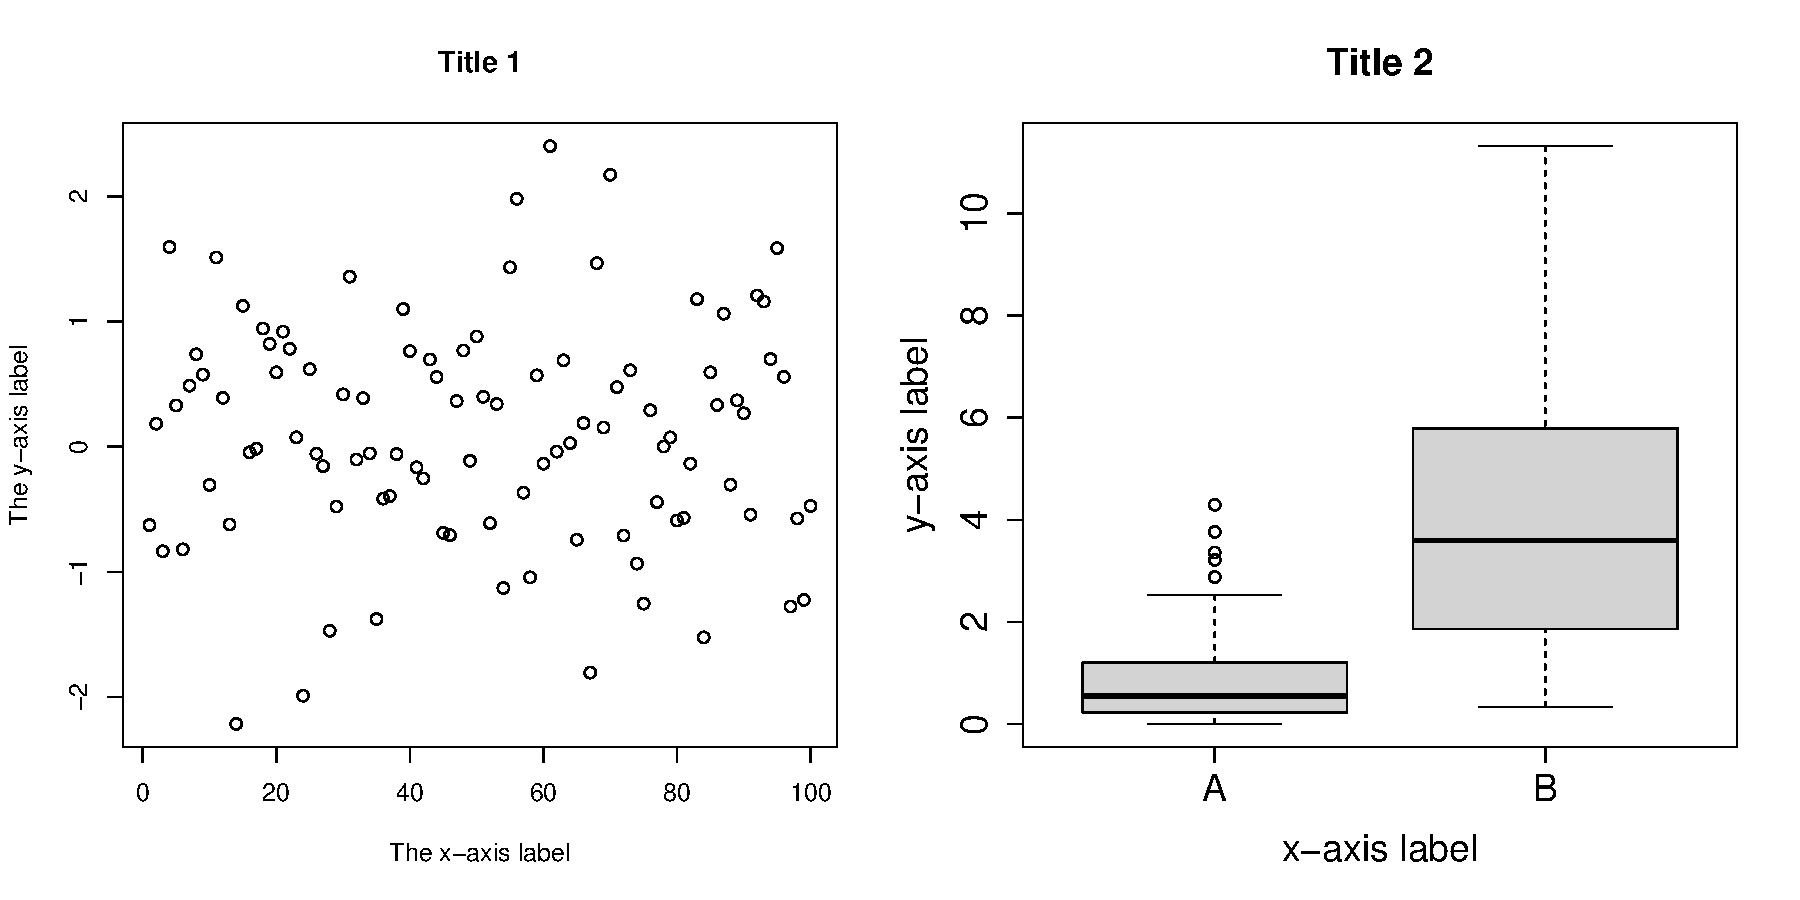
\includegraphics[width=0.9\textwidth]{assets/fig1.pdf}
    \caption{An example scatterplot (left) and box plot (right).}
    \label{fig:axis-label-example}
\end{figure}

\newpage

\section{Tables}\label{sec:tables}

\begin{table}[ht]
\centering
\begin{tabular}{rr}
  \hline
    $z$& $\textrm{P}(Z < z)$ \\
  \hline
    1.281& 0.900\\
    1.645& 0.950\\
    1.960& 0.975\\
    2.326& 0.990 \\
    2.576& 0.995 \\
   \hline
\end{tabular}
    \caption{Partial table showing values of $z$ for $\textrm{P}(Z < z)$, 
    where $Z$ has a standard normal distribution.}
    \label{tab:normal}
\end{table}

\newpage

\section{Proofs}\label{sec:proofs}

\begin{proof} \label{prf:obs-generation}
    (\hyperref[prop:obs-generation]{Proposition \ref{prop:obs-generation}}).
    Given:
    \begin{align*}
        \mathbf{X}_t \mid \mathbf{X}_0 = \mathbf{x}_0 \sim \mathcal{N}(c_t\cdot\mathbf{x}_0, d_t^2\cdot\mathbf{I}_{d_x}) \\
        \mathbf{Y}_t \mid \mathbf{X}_t = \mathbf{x}_t \sim \mathcal{N}(A\mathbf{x}_t, \sigma_y^2c_t^2\cdot\mathbf{I}_{d_y})
    \end{align*}
    We have:
    \begin{align*}
        \EE{\mathbf{Y}_t \mid \mathbf{X}_0} &= \EE{\EE{\mathbf{Y}_t \mid \mathbf{X}_t} \mid \mathbf{X}_0} \\
        &= \EE{A\mathbf{X}_t \mid \mathbf{X}_0} \\
        &= A\EE{\mathbf{X}_t \mid \mathbf{X}_0} \\
        &= c_t\cdot A\mathbf{X}_0
    \end{align*}
    and
    \begin{align*}
        \VV{\mathbf{Y}_t \mid \mathbf{X}_0} &= \EE{\VV{\mathbf{Y}_t \mid \mathbf{X}_t} \mid \mathbf{X}_0} + \VV{\EE{\mathbf{Y}_t \mid \mathbf{X}_t} \mid \mathbf{X}_0} \\
        &= \EE{\sigma_y^2c_t^2\cdot \mathbf{I}_{d_y} \mid \mathbf{X}_0} + \VV{A\mathbf{X}_t \mid \mathbf{X}_0} \\
        &= \sigma_y^2c_t^2\cdot \mathbf{I}_{d_y} + A\VV{\mathbf{X}_t \mid \mathbf{X}_0}A^\top \\
        &= \sigma_y^2c_t^2\cdot \mathbf{I}_{d_y} + d_t^2\cdot AA^\top
    \end{align*}
    Hence:
    \begin{equation*}
        \mathbf{Y}_t \mid \mathbf{X}_0 = \mathbf{x}_0 \sim \mathcal{N}(c_t\cdot A\mathbf{x}_0, \sigma_y^2c_t^2\cdot \mathbf{I}_{d_y} + d_t^2\cdot AA^\top)
    \end{equation*}
    But we note that $\mathbf{Y} = A\mathbf{X}_0$. Hence:
    \begin{equation*}
        \mathbf{Y}_t \mid \mathbf{Y} = \mathbf{y} \sim \mathcal{N}(c_t\cdot \mathbf{y}, \sigma_y^2c_t^2\cdot \mathbf{I}_{d_y} + d_t^2\cdot AA^\top)
    \end{equation*}
\end{proof}

\begin{proposition}[Gaussian-Gaussian Exactness for Linear Observations] \label{prop:gaussian-exact}
    Suppose
    \begin{align*}
        \mathbf{X}_{t} \mid \mathbf{X}_{t+1} &\sim \mathcal{N}\left( \mathbf{\mu}_{t+1}(\mathbf{x}_{t+1}), \Sigma_{t+1} \right)  \\
        \mathbf{Y}_{t} \mid \mathbf{X}_{t} = \mathbf{x}_{t} &\sim \mathcal{N}\left( A\mathbf{x}_{t}, \Xi_{t} \right)
    \end{align*}
    Consider some proposal:
    \begin{align*}
        p_{t}(\mathbf{x}_{t} \mid \mathbf{y}_{t}, \mathbf{x}_{t+1}) \propto p_{t}(\mathbf{x}_{t} \mid \mathbf{x}_{t+1})g_{t}(\mathbf{y}_{t} \mid \mathbf{x}_{t})
    \end{align*}
    Then:
    \begin{align*}
        \mathbf{Y}_{t} \mid \mathbf{X}_{t+1} = \mathbf{x}_{t+1} \sim \mathcal{N}\left( A\mu_{t+1}, \Xi_{t} + A\Sigma_{t+1}A^\top \right) 
    \end{align*}
\end{proposition}
\begin{proof}
    By Gaussian conjugacy, it immediately follows that:
    \begin{align*}
        \mathbf{X}_{t} \mid \mathbf{Y}_{t} = \mathbf{y}_{t}, \mathbf{X}_{t+1} = \mathbf{x}_{t+1} &\sim \mathcal{N}\left( \mu_{t+1}^P, \Sigma_{t+1}^P \right) 
    \end{align*}
    where
    \begin{align*}
        \mu_{t+1}^P &= \Sigma_{t+1}^P\left( \Sigma_{t+1}^{-1}\mu_{t+1}(\mathbf{x}_{t+1}) + A^\top\Xi_{t}^{-1}\mathbf{y}_{t} \right) \\
        \Sigma_{t+1}^P &= \left( \Sigma_{t+1}^{-1} + A^\top \Xi_{t}^{-1}A \right)^{-1}
    \end{align*}
    The normalizing constant of the proposal is:
    \begin{align*}
        \int p_{t}(\mathbf{x}_{t} \mid \mathbf{x}_{t+1})g_{t}(\mathbf{y}_{t} \mid \mathbf{x}_{t}) \, d\mathbf{x}_{t} &= g_{t}(\mathbf{y}_{t} \mid \mathbf{x}_{t+1})
    \end{align*}
    Note that:
    \begin{align*}
        \mathbb{E}\left\{ \mathbf{Y}_{t} \mid \mathbf{X}_{t+1} \right\} &= \mathbb{E}\left\{\mathbb{E}\left\{\mathbf{Y}_{t} \mid \mathbf{X}_{t}\right\} \mid \mathbf{X}_{t+1}\right\} &\dots\text{tower property} \\
        &= \mathbb{E}\left\{A\mathbf{X}_{t} \mid \mathbf{X}_{t+1}\right\} \\
        &= A\mathbb{E}\left\{\mathbf{X}_{t} \mid \mathbf{X}_{t+1}\right\} \\
        &= A\mu_{t+1}(\mathbf{X}_{t+1}) \\
        \mathbb{V}\left\{\mathbf{Y}_{t} \mid \mathbf{X}_{t+1}\right\} &= \mathbb{E}\left\{\mathbb{V}\left\{\mathbf{Y}_{t} \mid \mathbf{X}_{t}\right\} \mid \mathbf{X}_{t+1}\right\} + \mathbb{V}\left\{\mathbb{E}\left\{\mathbf{Y}_{t} \mid \mathbf{X}_{t}\right\} \mid \mathbf{X}_{t+1}\right\} &\dots \text{total variance} \\
        &= \mathbb{E}\left\{\Xi_{t} \mid \mathbf{X}_{t+1}\right\} + \mathbb{V}\left\{A\mathbf{X}_{t} \mid \mathbf{X}_{t+1}\right\} \\
        &= \Xi_{t} + A\mathbb{V}\left\{\mathbf{X}_{t} \mid \mathbf{X}_{t+1}\right\}A^{\top} \\
        &= \Xi_{t} + A\Sigma_{t+1}A^{\top}
    \end{align*}
    Since $\mathbf{Y}_{t}$ is an affine transformation, it follows then that:
    \begin{align*}
        \mathbf{Y}_{t} \mid \mathbf{X}_{t+1} = \mathbf{x}_{t+1} \sim \mathcal{N}\left( A\mu_{t+1}, \Xi_{t} + A\Sigma_{t+1}A^\top \right) 
    \end{align*}
\end{proof}

\section{Extra}

\begin{remark}[DDIM Representation]
    Under DDIM:
    \begin{equation*}
        u_t = \sqrt{\alpha_{t-1}} \quad
        v_t = -\sqrt{1 - \overline{\alpha}_{t-1} - \sigma_t^2}\sqrt{1 - \overline{\alpha}_t} \quad
        w_t = \sigma_t
    \end{equation*}
    with $\{\sigma_t\}_{t=1}^T$ an arbitrary conditional variance sequence. It's common to consider:
    \begin{equation*}
        \sigma_t(\eta) = \eta\sqrt{\frac{1 - \alpha_{t-1}}{1 - \alpha_t}}\sqrt{1 - \frac{\alpha_t}{\alpha_{t-1}}},\quad \eta \in [0,1]
    \end{equation*}
    with $\eta=1$ ultimately reducing $u_t, v_t, w_t$ to the DDPM values, and $\eta=0$ corresponding
    to deterministic generation \parencite{songDenoisingDiffusionImplicit2020}.
\end{remark}

\begin{remark}[Time Respacing]
    One of the remarkable features of the DDIM algorithm is it enabling \emph{time re-spacing}
    whereby we can sample from the backwards process in fewer time-steps. In this paper, we don't
    consider such re-spacing though in principle our methodology does not prohibit it.
\end{remark}
